\documentclass[11pt]{article}
\usepackage[utf8]{inputenc}
\usepackage[french]{babel}
\usepackage{graphicx}
\usepackage{epstopdf}
\usepackage[T1]{fontenc}
\usepackage{amsmath}
\usepackage{amsfonts}
\usepackage{amssymb}
\def\N{\mathbb N}
\def\R{\mathbb R}
\def\Q{\mathbb Q}
\def\Z{\mathbb Z}
\usepackage{parskip}
%\setlength{\parskip}{0.6mm}
\setlength{\parskip}{\baselineskip}
\newcommand{\comment}[1]{}

\begin{document}
\title{EXAMEN LICENCE 2, MODULE I31, 15-12-2016}
%\author{LICENCE 2, MODULE I31}
\date{}

\maketitle
\newif\ifcorrige
%\corrigetrue
\corrigefalse

\newcommand{\smallbullet}{\,\begin{picture}(-1,1)(-1,-3)\circle*{2}\end{picture}\ }

%\fbox{\parbox{0.95\linewidth}{LA COPIE EST NOTEE ZERO DES QU'IL Y A UN PROGRAMME.}}
%%\bigskip

REPONDEZ AUX QUESTIONS DANS L'ORDRE. 

NUMEROTEZ VOS QUESTIONS.

ECRIVEZ LISIBLEMENT.

AUCUN ALGORITHME, ET AUCUN PROGRAMME.

\section{Quizz (sur 10 points)}
1. Citer 6 structures de données.
 
\ifcorrige
{\it Solution~: pile, liste, tas, file, arbre, graphe, table de hachage, tableau}
\else
\fi

 
2. En détaillant les trois étapes, triez avec la méthode du tri par base ("radix sort") les nombres~:
$321, 231, 123, 221, 113, 213, 131, 311$.

 
3. Le graphe $G$ est ci-dessous. A partir de ses composantes fortement connexes, dessinez son graphe réduit, $R$. Indiquez sur chaque sommet de $R$ quels sont les sommets correspondant dans $G$.
\begin{center}
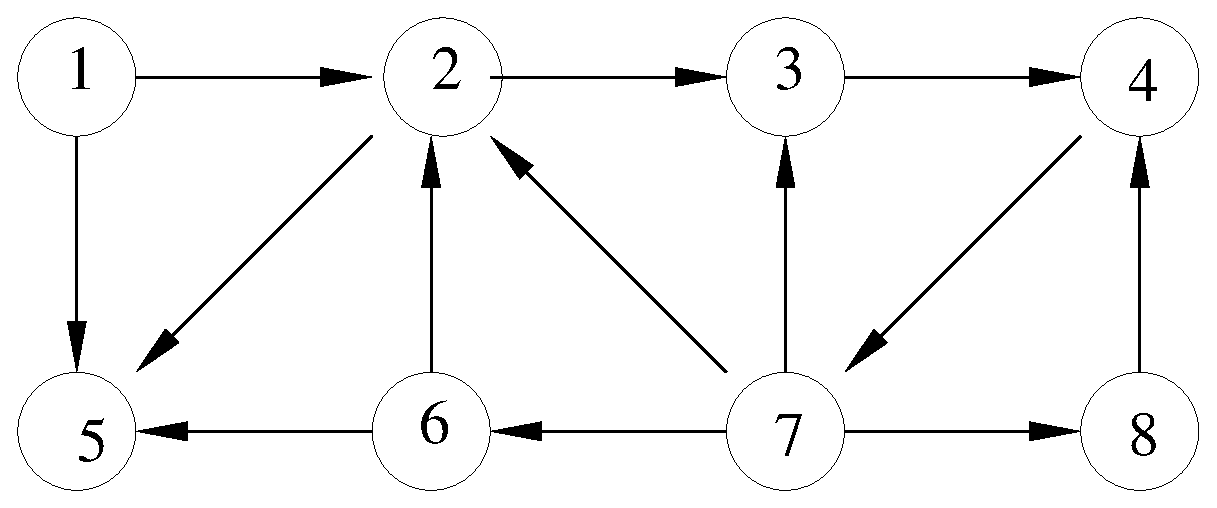
\includegraphics[width=0.6\linewidth]{scc.eps}
\end{center}

 
\ifcorrige
{\it Solution.}
\begin{center}
\includegraphics[width=0.6\linewidth]{scc_bis.eps}
\end{center}
\else
\fi

 
4.  Quelle est la complexité du tri rapide (ou {\it quicksort}) d'un tableau de $n$ éléments~? Quelle est la formule récusive pour $T(n)$~? La méthode n'est pas demandée.
Répondre en 1 ligne.

 
\ifcorrige
{\it Solution. $O(n)$. Utiliser le tri rapide (quicksort) "d'un seul côté".
La formule est donc~: $T(n)=T(n/2)+n$.
}
\else
\fi

\comment{
5. Peut-on utiliser l'algorithme de Dijkstra quand les arcs portent des coûts négatifs~? Même question pour l'algorithme de  Ford (ou Ford-Bellman, ou Bellman-Ford, ou Bellman–Ford–Moore\footnote{En fait, Alfonso Shimbel l'a proposé avant, en 1955 [Wikipedia].})~? %% S'il peut y en avoir, peut-il y avoir des circuits de coût globalement négatif~?  
\ifcorrige
{\it Solution. Non pour Dijkstra. Oui pour Ford.}
\else
\fi
}


\comment{
6. Un graphe orienté a des arcs étiquetés avec des coûts négatifs. Existe-t-il forcément des circuits de coût global négatif~? Si oui, prouvez-le~; sinon, prouvez-le.
%
\ifcorrige
{\it Solution. Non, pas forcément. Un contre-exemple suffit pour le prouver. Le graphe qui ne contient que l'arc~: $a\rightarrow b$ de coût $-1$ n'a pas de cycle donc pas de cycle de coût global négatif. Autre contre-exemple~: le graphe avec deux arcs~: $a\rightarrow b$ de coût $-1$ et $b\rightarrow a$ de coût 2. 
}
\else
\fi
}
 
5. Rappelez, par une formule, la définition de la date au plus tôt et de la date au plus tard dans un graphe orienté sans cycle où les arcs sont étiquetés par des durées. N'oubliez pas de cas.  %Quand un sommet est-il critique~? Quel problème sur des séquences a été réduit  à un problème de chemin critique~?

\ifcorrige {\it Solution.
$$ \mbox{tôt}(s) = 0 \mbox{ quand } s \mbox{ est une source.} $$
$$ \mbox{tôt}(s) = \max_{r \;:\; \exists r\rightarrow s} \mbox{tôt}(r)+ \mbox{durée}(r\rightarrow s)$$
$$ \mbox{tard}(s) = \mbox{tôt}(s)  \mbox{ quand } s \mbox{ est un puits.} $$
$$ \mbox{tard}(s) = \min_{t \;:\; \exists s\rightarrow t} \mbox{tard}(t) - \mbox{durée}(s\rightarrow t)$$
}
\else
\fi

 
6. Le chemin critique est-il un chemin le plus court dans le graphe de la question précédente~?

\ifcorrige
{\it Solution. Non, c'est le chemin le plus long entre la source (ou les sources) et le puits (ou les puits).
}
\else
\fi

 
7. Dans le  graphe de la figure ci-dessous, $G_{u,v}$ est le coût ou la longueur de l'arc $u\rightarrow v$. Quel est la longueur du chemin le plus court, en 2 arcs, de $a$ vers $c$~? 
% Comme sommet intermédiaire, utilisez $k$ (et donc $G_{ak}$, $G_{kc}$) ou $b$ (et donc $G_{ab}$, $G_{bc}$). 
Répondre par une formule en 1 ligne.
Utiliser une variable pour le sommet intermédiaire, par exemple $\sum_c G_{ab}\times G_{bc}$ (attention, cette formule est fausse).
Pour que votre formule soit correcte quand il n'existe pas d'arc $u\rightarrow v$, que doit valoir $G_{u,v}$ (quand  il n'existe pas d'arc $u\rightarrow v$)~?
Répondre en une ligne.

\begin{center}
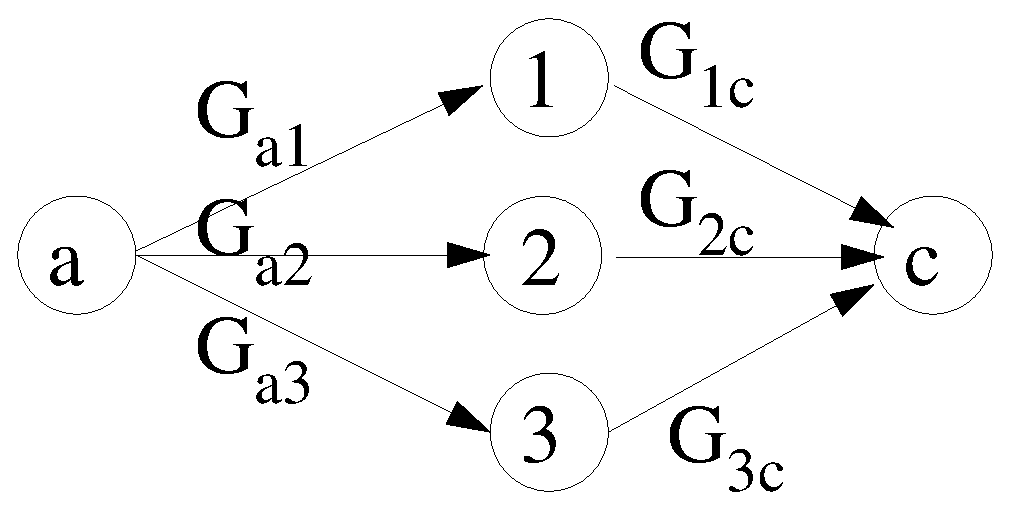
\includegraphics[width=0.5\linewidth]{graphe.eps}
\end{center}
\ifcorrige {\it Solution. La longueur du chemin le plus court est $\min_k G_{ak}+G_{kc}$. Quand $u\rightarrow v$ n'existe pas, $G_{u,v}=\infty$.}
\else\fi

 
8. (suite)  $G_{u,v}$ est ici  la probabilité de survivre
(ou de bon fonctionnement) en parcourant l'arc
$u\rightarrow v$. Quelle est la probabilité de survivre du  chemin le plus sûr, en 2 arcs,
de $a$ vers $c$~?  Répondre par une formule en 1 ligne.
Pour que votre formule soit correcte quand il n'existe pas d'arc $u\rightarrow v$, que doit va
loir $G_{u,v}$~?
Répondre en une ligne.
Cette dernière question est posée car il est essentiel de savoir initialiser  les variables.
 

\ifcorrige {\it Solution.
La probabilité de survie du chemin le moins risqué est
$\max_k G_{ak}\times G_{k,c}$.
Si $u\rightarrow v$ n'existe pas, alors $G_{u,v}=0$.}
\else\fi

 
9. (suite) $G_{u,v}$ est ici   la probabilité de mourir (ou de tomber en panne) en parcourant l'arc
$u\rightarrow v$. Quelle est la probabilité de mourir dans le chemin en 2 arcs le plus sûr  de $a$ vers $c$~? Répondre par une formule en 1 ligne.
Pour que votre formule soit correcte quand il n'existe pas d'arc $u\rightarrow v$, 
que doit valoir $G_{u,v}$~?
Répondre en une ligne.

\ifcorrige {\it Solution.
La probabilité de mort du chemin le moins risqué est
$\min_k (1-(1-G_{ak})(1-G_{k,c}))= G_{ak}+G_{k,c}-G_{ak}G_{k,c}$.
Si $u\rightarrow v$ n'existe pas, alors  $G_{u,v}=1$.}
}
\else\fi
 

10. (suite)  $G_{u,v}$ est  ici la capacité de l'arc $u\rightarrow v$~; en termes imagés,
$G_{u,v}$ est le diamètre d'un tuyau qui descend de $u$ à $v$, dans lequel vont pouvoir rouler ou chuter  des billes de diamètre au plus $G_{u,v}$.
Quelle est la capacité du chemin de plus grande capacité,
en 2 arcs, de $a$ vers $c$~?
Répondre par une formule en 1 ligne.
Pour que votre formule soit correcte quand il n'existe pas d'arc $u\rightarrow v$, 
que doit valoir $G_{u,v}$~?
Répondre en une ligne.

Remarque. Les questions 8, 9, 10 n'ont pas forcément été vues en cours. Elles permettent de prouver que vous savez lire, comprendre ce que vous lisez, et rédiger, autrement dit
que vous pouvez  programmer.

\ifcorrige {\it Solution.
La capacité maximale est 
$\max_k ( min( G_{ak}, G_{kc} ))$.
Si $u\rightarrow v$ n'existe pas, alors   $G_{u,v}=0$.
}
\else\fi




\section{La méthode de Newton (sur 5 points)}
 
1. La fonction $f$ est définie par $f(x)=x^3-9$. Donnez $f'(x)$.
Donnez  $N(x)$, où $N$ est la fonction de Newton associée à $f$.
 
\ifcorrige
{\it Solution. $f'(x)=3x^2$ }
\else\fi

\ifcorrige
{\it Solution. $N(x)=x - f(x)/f'(x)= x - (x^3-9)/(3x^2)=2x/3 + 3/(x^2)$
}
\else\fi


2. Expliquez à quoi elle sert, en 1 ligne au plus.
 
\ifcorrige
{\it Solution. A résoudre $f(x)=0$, en trouvant un point fixe de $N$.
}
\else\fi

 
%%3. Donnez $N'(x)$.


3.  Calculez $N(1/2), N(1), N(2), N(3)$ et dessinez   avec soin la courbe $(x, N(x))$ pour $0 < x \le 3$.
Dessinez aussi la droite d'équation $y=x$.
En partant de $x_0=1$, dessinez 
le chemin suivi par la méthode de Newton (les valeurs exactes ne sont pas demandées).
 
4. La méthode de la sécante est une variante de la méthode de Newton, où
$f'(x)$ est remplacée par $f'(v)$. Calculez $f'(2)$ et indiquez ce 
que vaut la fonction sécante $S(x)$ pour  $v=2$. 
Dessinez  la courbe $(x, S(x))$ pour $-1 \le x \le 3$.
Dessinez  aussi la droite d'équation $y=x$.
En partant de $x_0=1$, dessinez
le chemin suivi par la méthode de la sécante
(Les valeurs exactes ne sont pas demandées).
 
5. Quand $|N'(x)|< 1$, ou $|S'(x)| < 1$, la convergence est garantie. Résolvez
$S'(x)=1$, ainsi que $S'(x)= -1$ (vous pouvez  contrôler vos solutions sur votre dessin). 


\ifcorrige
{\it Réponse. La dérivée de $f$ est $f'(x)=3x^2.$

La fonction de Newton est~: $N(x)= x - f(x)/f'(x) = x - (x^3-9)/(3x^2)$.

La sécante est $S(x)= x - (x^3-9)/12$, et $S'(x)=1-3x^2/12=1-x^2/4$.

$S'(x)=1-x^2/4=1 \Rightarrow x=0$

$S'(x)=1-x^2/4=-1  \Rightarrow x =\sqrt{}=2\sqrt{2}$

% $S'([2, 5/2])= 1 - [4, 25/4]/4= [-9/16, 0]$ a donc une valeur absolue inférieure à 1. Donc $[2, 5/2]$ contient au plus une racine.
}
\else
\fi

{
\section{Algorithme d'Euclide généralisé (2 points)}
Utilisez  l'algorithme d'Euclide généralisé
pour calculer le PGCD $g$ de $a=104$ et $b=39$. Outre le PGCD, vous devez
aussi calculer deux entiers relatifs $u$ et $v$ tels que $a u + b v=g$ (coefficients de Bezout). 
Utilisez une présentation sous forme de tableau, avec des colonnes $a$, $b$, $q$, $r$, $u$, $v$, $g$, comme en TD ($q=\lfloor a/b\rfloor, r=a \mod b$).

En fait, il existe une infinité de solution pour $u, v$, qu'on peut paramétrer par $t\in \Z$~: donnez une expression paramétrée  $u(t)$ et $v(t)$ (il y a deux solutions).
}

\ifcorrige
{\it Réponse.
$$\begin{array}{|c|c|c|c|c|c|c|}
\hline
a & b & r & q & g & u & v \\
\hline
104 & 39 & 26 & 2 & 13 & -1 & 3 \\
39 & 26 & 13 & 1 & 13 & 1 & -1 \\
26 & 13 & 0 & 2 & 13 & 0 & 1 \\
13 & 0 & * & * & 13 & 1 & 0 \\
\hline
\end{array}
$$
Donc: $u=-1, v=3, g=13$, et $au+bv=104\times  (-1) + 39\times 3= 13=g$.
Divisons par $g$~: $8\times (-1) + 3\times 3=1$. Alors pour tout $t\in \Z$,
$8\times (-1+3t) + 3\times (3-8t)=1$, donc, en multipliant par $g=13$~: $104\times (-1+3t) + 39\times (3-8t)=13$.
Donc $u=-1+3t$, $v=3-8t$. Bien sûr, $u=-1-3t$, $v=3+8t$ est aussi correct.
}
\else\fi

\section{Produit optimal de matrices (3 points)}
La matrice $A$ a 1 ligne, 1000 colonnes.
La matrice $B$ a 1000 lignes, 2 colonnes.
La matrice $C$ a 2 lignes, 1000 colonnes.
 

1. Quel est le nombre de lignes et de colonnes de $(AB)C$ et de $A(BC)$~?
Quel est le nombre de multiplications pour calculer $(AB)C$, et pour calculer $A(BC)$~?

2. Quel est le nom de l'algorithme vu en cours pour trouver le parenthésage optimal~?

 

3. Donnez la formule (récursive) du coût optimal $C(i, j)$ (avec $i\le j$) pour multiplier les matrices
$M_i, \ldots M_j$ avec ce type d'algorithme. Vous noterez $l_i, c_i$ le nombre de lignes et de colonnes de la matrice $M_i$.

\ifcorrige {\it  Réponse.
$(AB)C=A(BC)=ABC$ a 1 ligne et 1000 colonnes.
Pour calculer $(AB)C$ il faut 2000+2000 multiplications de nombres flottants.
Pour calculer $A(BC)$, il en faut $3\times 10^6$.
Nous avons utilisé la programmation dynamique pour trouver le parenthésage optimal. La formule est~:
$$C(i, j)= 0 \mbox{ si } i=j$$
$$C(i, j)= \min_{k=i}^{j-1} C(i, k) + C(k+1, j) + l_i\times c_k\times c_j $$
}
\else\fi

\end{document}

\section{Séquence commune la plus longue}
Dessinez le graphe permettant de trouver la séquence commune la plus longue
entre $ABACAB$ et $ACBCBC$. Dessinez $ABACAB$ horizontalement, et  $ACBCBC$ verticalement et ascendante~: autrement dit tous les arcs doivent monter de gauche à droite. Il n'est pas nécessaire de tracer les arcs de transitivité. Tracer le (ou les) chemin(s) critique(s).
 
\section{Célébrité}
$n$ personnes, numérotées de 1 à $n$, sont réunies. Par définition, une célébrité est quelqu'un que tout le monde connaît, mais qui ne connaît personne (à part elle-même). La fonction connaît( $a, b$) dit si $a$ connaît $b$. 
On appelle cette fonction un oracle.

Combien peut-il y avoir de célébrités au maximum, parmi $n$ personnes~? (1 ligne)

\ifcorrige {\it Une célébrité au plus. }
\else\fi

Si $a$ connaît $b$ (avec $a\neq b$), l'un des deux ne peut être une célébrité~; lequel~? (répondre en 1 ligne)

\ifcorrige{\it $a$ ne peut pas être une célébrité.}
\else\fi

Si $a$ ne connaît pas $b$ (avec $a\neq b$), l'un des deux ne peut être une célébrité~; lequel~? (répondre en 1 ligne)

\ifcorrige{\it $b$ ne peut pas être une célébrité.}\else\fi

Combien de questions faut-il poser à l'oracle
pour éliminer $n-1$ candidats à la célébrité~?

\ifcorrige{\it $n-1$}\else\fi

Quand il ne reste plus qu'un seul candidat, combien de questions faut-il poser à l'oracle
pour décider si ce candidat est une célébrité ou non~? 

\ifcorrige{\it $2n-2$ si c'est une célébrité, et moins sinon.}
\else\fi




\end{document}
\section{Sous-ensembles de nombres non consécutifs}
Un ensemble d'entiers est dit non consécutif s'il ne contient pas deux entiers consécutifs ($n$ et $n+1$ sont consécutifs, pour $n\in \N$).
Soit  $F_n$ l'ensemble des sous-ensembles de nombres entiers, non consécutifs, et compris entre 1 et $n$ (0 est inutilisé).  $F_n$ contient $f_n=|F_n|$ ensembles.
Par exemple~:

\indent $F_0=\{ \emptyset \}$,  $f_0=1 $, \\
\indent $F_1= \{ \emptyset, \{1\}\}$, $f_1= 2$,\\
\indent $F_2= \{ \emptyset, \{1\}, \{2\} \}$, $f_2=3$,\\
\indent $F_3= \{ \emptyset, \{1\}, \{2\}, \{3\}, \{1, 3\}\}$, $f_3=5 $,\\
\indent $F_4= \{ \emptyset, \{1\}, \{2\}, \{3\}, \{4\},  \{1, 3\}, \{1, 4\}, \{2, 4 \}\}$, $f_4=8$.


Que semble valoir $f_n$~? (réponse en une ligne).

\ifcorrige {\it Réponse. $f_n$ est le $n$ ième nombre de Fibonacci. }
\else\fi


Proposez une définition récursive de $F_n$ (réponse en une ligne).
Vous pouvez utiliser la notation suivante~:
$$F_k \oplus v= \bigcup_{E\in F_k} \{v\} \cup E$$
Par exemple,
$$F_2 \oplus 4= \{ \emptyset, \{1\}, \{2\} \} \oplus 4= \{ \{4\}, \{1,4\},  \{2, 4\}  \}$$

\ifcorrige {\it Solution.
$$ n>1 \Rightarrow F_n= F_{n-1} \cup (F_{n-2} \oplus n)$$
}
\else\fi

\section{3-5-8}
Un problème de transvasement  typique est celui ci. 
Trois récipients non gradués ont des capacités de 3 litres, 5  et 8 litres.
Initialement, ils contiennent respectivement 0,  3 et 5 litres d'eau. Comment en transvasant les
récipients passer à 0, 4 et 4 litres d'eau dans les récipients de 3, 5 et 8~?
Comme les récipients ne sont pas gradués, quand on transvase un récipient $a$
dans un récipient $b$, 
il faut s'arrêter dès que $a$ est vide ou que $b$ est plein. 

Il ne vous est pas demandé de résoudre ce problème,  mais de 
proposer une méthode capable de résoudre ce type de casse-tête.
Répondez en cinq lignes maximum. Votre réponse doit être {\it lisible et claire}.

\ifcorrige 
{\it Solution. Il faut trouver un chemin dans le graphe des états.
Chaque état $(a\le A, b\le B, c\le C)$ donne un sommet, et chaque transvasement
d'un état $e=(a, b, c)$ vers un état $e'=(a', b', c')$ donne un arc $e\rightarrow e'$ dans le graphe.
Le graphe n'est pas symétrique.
Le chemin peut être trouvé par "backtrack" (parcours en profondeur ou en largeur), ou par un calcul de chemin le plus court (en nombre d'arcs par exemple).
}
\else
\fi

\end{document}
